\documentclass[12pt]{article}

%   Sprache und Font
\usepackage{polyglossia}
\setmainlanguage{german}
\usepackage{fontspec}
\setmainfont{Free Helvetian}
\setsansfont{Free Helvetian}
\setmonofont{FreeMono}
\usepackage{csquotes}

\usepackage{graphicx}

%   Abbildungen müssen in einem Ordner "Abbildungen" liegen
\graphicspath{ {Abbildungen/} }
\usepackage{pdfpages}

\usepackage{etoolbox}
\AtBeginEnvironment{quote}{\small\setstretch{.25}}

\renewcommand{\familydefault}{\sfdefault}
\renewcommand\labelenumi{(\theenumi)}

\usepackage{tabularx}

%   Zitationsstil
\usepackage[style=authoryear-icomp,maxcitenames=2,backend=biber]{biblatex}
\addbibresource{bibliography.bib}

\usepackage{import}

%   Überschriften
\usepackage{titlesec}
\titlespacing\section{0pt}{12pt plus 4pt minus 2pt}{0pt plus 2pt minus 2pt}
\titlespacing\subsection{0pt}{12pt plus 4pt minus 2pt}{0pt plus 2pt minus 2pt}
\titlespacing\subsubsection{0pt}{12pt plus 4pt minus 2pt}{0pt plus 2pt minus 2pt}

\usepackage{setspace}
\definecolor{hgray}{gray}{0.5}

%   Styling der Aufzählungen
\usepackage{enumitem}
\setlist[itemize]{noitemsep, topsep=0pt}
\setlist[enumerate]{noitemsep, topsep=0pt}

%   Sinnvoll formatierte Links
\usepackage[hidelinks,
pdfpagelabels,
pdfstartview = FitH,
bookmarksopen = true,
bookmarksnumbered = true,
linkcolor = black,
plainpages = false,
hypertexnames = false,
citecolor = black] {hyperref}

%   Worttrennung
\usepackage{hyphenat}
\hyphenation{Kon-sis-tenz-pro-ble-me Ter-mi-no-lo-gie-pro-ble-me}


%   Seiteneinrichtung
\usepackage{geometry}
\geometry{
  left=2.5cm,
  right=2.5cm,
  top=2.5cm,
  bottom=2cm,
  bindingoffset=0mm
}


\makeatletter
\title{Evaluation der kommunikativen Usability von RWTH {\nobreak Online}}\let\Title\@title     %   Titel der Arbeit eintragen
\makeatother



\usepackage{fancyhdr}
\usepackage{afterpage}
\fancypagestyle{MRstyle}{
    \fancyhf{}
    \fancyhead[L]{\textit{\textcolor{hgray}{\Title}}}
    \fancyfoot[c]{\textcolor{hgray}{\thepage}}
}

\fancypagestyle{appendix}{
    \fancyhf{}
    \fancyhead[L]{\textit{\textcolor{hgray}{\Title}}}
    \fancyhead[R]{\textcolor{hgray}{\rightmark}}
    \fancyfoot[c]{\textcolor{hgray}{\thepage}}
}

\usepackage[hang]{footmisc}

\newcommand\fakesection[1]{% 
    \markboth{#1}{#1}}

\usepackage{parskip}
\DefineBibliographyStrings{german}{ 
   andothers = {{et\,al\adddot}},             
} 



% Das Dokument geht hier los:

\begin{document}
\pagestyle{MRstyle}
 
\setstretch{1.15}

\begin{titlepage}
    
    \large
    RWTH Aachen\\
    Institut für Sprach- und Kommunikationswissenschaft\\
    Professur für Textlinguistik und Technikkommunikation\\
    Prof. Dr. E.-M. Jakobs
    
    \vspace{5cm}
    \Large
    \doublespacing{
        \textit{Seminararbeit \\}
        \textbf{\Title}
    }
    
    \vspace{7cm}
    \normalsize
    \setstretch{1.2}
    vorgelegt von:\\
    Maximilian Röttgen (Matrikel-Nr.: 332048)\\ % Hier Name, Matr. Nr. etc. einfügen
    Martin Schmitz (Matrikel-Nr.: 320669)
    
    \vfill
    
    Aachen, \today    
\afterpage{\cfoot{\textcolor{hgray}{\thepage}}}
        
\end{titlepage}


\pagenumbering{Roman}

\tableofcontents
\clearpage
\pagenumbering{gobble}
\section*{Zusammenfassung}


\clearpage
\pagenumbering{arabic}
\section{Einleitung}
\import{Kapitel/}{01_einleitung.tex}


\clearpage
\section{Literatur}
\import{Kapitel/}{02_literatur.tex}


\clearpage
\section{Methodik}
\import{Kapitel/}{03_methodik.tex}


\clearpage
\section{Ergebnisse}
\import{Kapitel/}{04_ergebnisse.tex}


\clearpage
\section{Diskussion}
\import{Kapitel/}{05_diskussion.tex}


\clearpage
\section{Fazit}
\import{Kapitel/}{06_fazit.tex}


\clearpage
\pagenumbering{Roman}

\clearpage
\appendix
\pagestyle{appendix}

\label{att:Screeningbogen}
\fakesection{Screening Fragebogen}
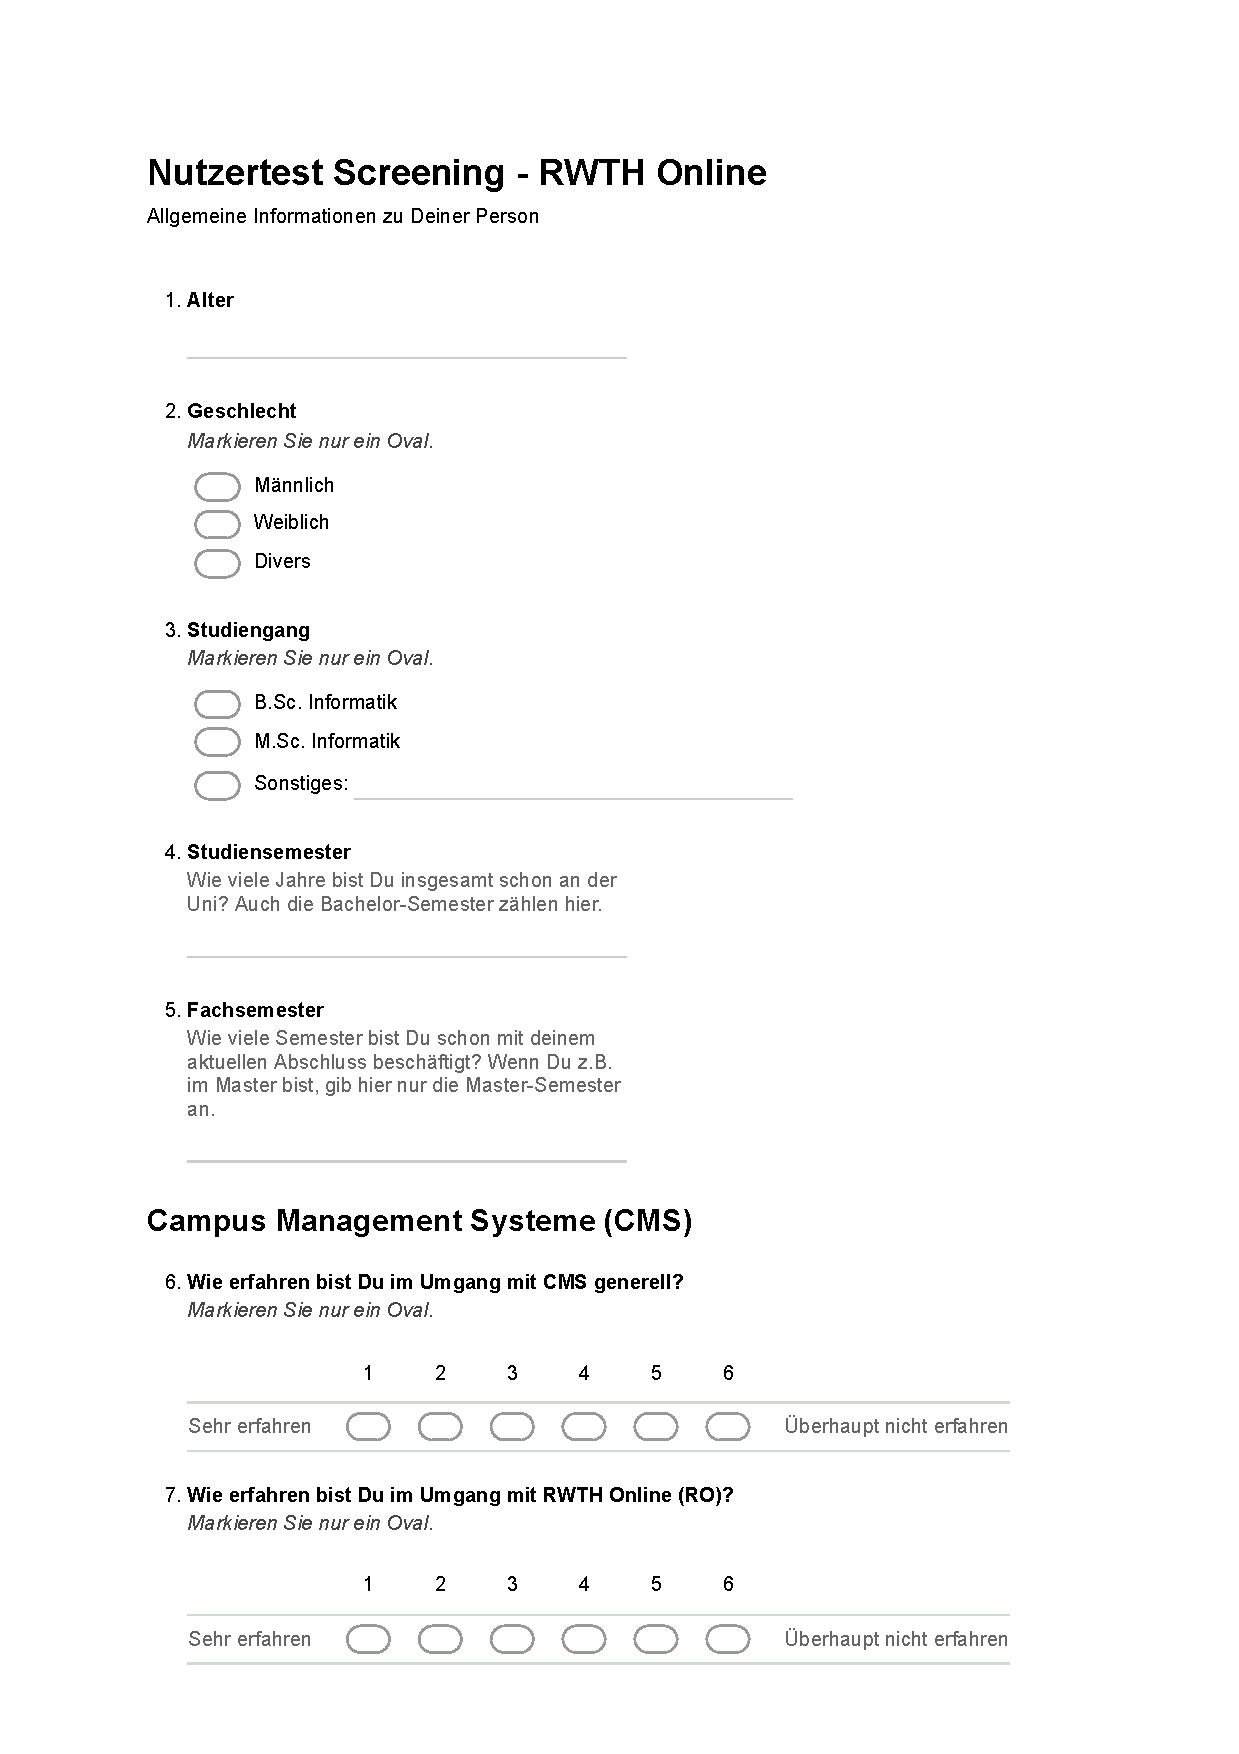
\includepdf[pages={1},scale=0.9,pagecommand={\section{Anhang}}]{Anhänge/Screening_Bogen.pdf}
\includepdf[pages={2},scale=0.9,pagecommand={}]{Anhänge/Screening_Bogen.pdf}
\includepdf[pages={3},scale=0.9,pagecommand={}]{Anhänge/Screening_Bogen.pdf}

\label{att:Drehbuch}
\fakesection{Drehbuch Nutzerstudie}

\includepdf[pages={1},scale=0.9,pagecommand={}]{Anhänge/Drehbuch.pdf}

\includepdf[pages={2},scale=0.9,pagecommand={}]{Anhänge/Drehbuch.pdf}

\includepdf[pages={3},scale=0.9,pagecommand={}]{Anhänge/Drehbuch.pdf}

\includepdf[pages={4},scale=0.9,pagecommand={}]{Anhänge/Drehbuch.pdf}

\includepdf[pages={5},scale=0.9,pagecommand={}]{Anhänge/Drehbuch.pdf}

\includepdf[pages={6},scale=0.9,pagecommand={}]{Anhänge/Drehbuch.pdf}

\includepdf[pages={7},scale=0.9,pagecommand={}]{Anhänge/Drehbuch.pdf}


\section{Literaturverzeichnis}
\pagestyle{MRstyle}
\setcounter{biburllcpenalty}{7000}
\setcounter{biburlucpenalty}{8000}
\printbibliography
\pagebreak

\pagestyle{plain}
\pagenumbering{gobble}
%\includepdf[pagecommand={}]{Eidesstattliche_Versicherung.pdf}

\end{document}
